\documentclass{standalone}
\usepackage{tikz}
\usetikzlibrary{shapes.geometric, arrows}

\tikzstyle{startstop} = [rectangle, rounded corners, minimum width=3cm, minimum height=1cm,text centered, draw=black, fill=red!30]
\tikzstyle{process} = [rectangle, minimum width=3cm, minimum height=1cm, text centered, draw=black, fill=orange!30]
\tikzstyle{decision} = [diamond, minimum width=3cm, minimum height=1cm, text centered, draw=black, fill=green!30]
\tikzstyle{arrow} = [thick,->,>=stealth]

\begin{document}

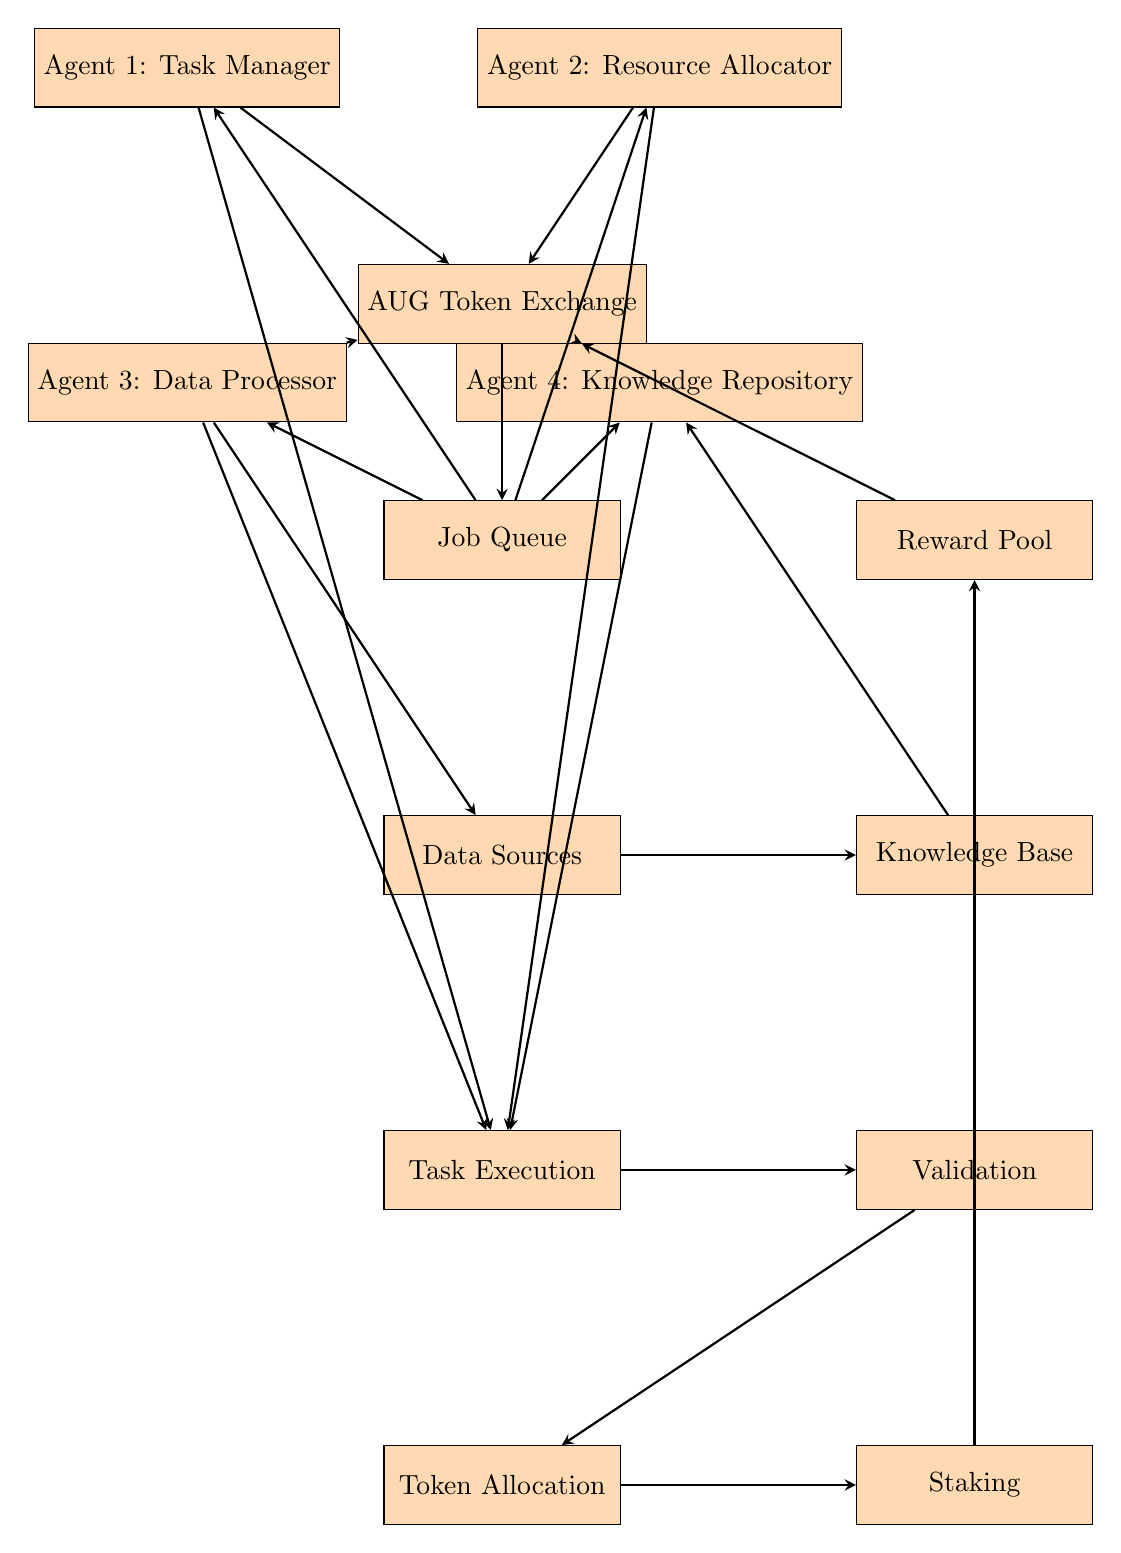
\begin{tikzpicture}[node distance=2cm]

    % Nodes
    \node (augTokenExchange) [process] {AUG Token Exchange};
    \node (jobQueue) [process, below of=augTokenExchange, yshift=-1cm] {Job Queue};
    \node (rewardPool) [process, right of=jobQueue, xshift=4cm] {Reward Pool};
    
    \node (agent1) [process, above of=augTokenExchange, yshift=1cm, xshift=-4cm] {Agent 1: Task Manager};
    \node (agent2) [process, right of=agent1, xshift=4cm] {Agent 2: Resource Allocator};
    \node (agent3) [process, below of=agent1, yshift=-2cm] {Agent 3: Data Processor};
    \node (agent4) [process, right of=agent3, xshift=4cm] {Agent 4: Knowledge Repository};
    
    \node (dataSources) [process, below of=jobQueue, yshift=-2cm] {Data Sources};
    \node (knowledgeBase) [process, right of=dataSources, xshift=4cm] {Knowledge Base};
    
    \node (taskExecution) [process, below of=dataSources, yshift=-2cm] {Task Execution};
    \node (validation) [process, right of=taskExecution, xshift=4cm] {Validation};
    
    \node (tokenAllocation) [process, below of=taskExecution, yshift=-2cm] {Token Allocation};
    \node (staking) [process, right of=tokenAllocation, xshift=4cm] {Staking};

    % Arrows
    \draw [arrow] (agent1) -- (augTokenExchange);
    \draw [arrow] (agent2) -- (augTokenExchange);
    \draw [arrow] (agent3) -- (augTokenExchange);
    \draw [arrow] (agent4) -- (augTokenExchange);
    
    \draw [arrow] (augTokenExchange) -- (jobQueue);
    \draw [arrow] (jobQueue) -- (agent1);
    \draw [arrow] (jobQueue) -- (agent2);
    \draw [arrow] (jobQueue) -- (agent3);
    \draw [arrow] (jobQueue) -- (agent4);
    
    \draw [arrow] (agent3) -- (dataSources);
    \draw [arrow] (dataSources) -- (knowledgeBase);
    \draw [arrow] (knowledgeBase) -- (agent4);
    
    \draw [arrow] (agent1) -- (taskExecution);
    \draw [arrow] (agent2) -- (taskExecution);
    \draw [arrow] (agent3) -- (taskExecution);
    \draw [arrow] (agent4) -- (taskExecution);
    
    \draw [arrow] (taskExecution) -- (validation);
    \draw [arrow] (validation) -- (tokenAllocation);
    \draw [arrow] (tokenAllocation) -- (staking);
    \draw [arrow] (staking) -- (rewardPool);
    \draw [arrow] (rewardPool) -- (augTokenExchange);

\end{tikzpicture}

\end{document} 